\documentclass[addpoints,12pt]{exam}
    \usepackage[a4paper]{geometry}
    \usepackage{enumitem}
    \usepackage{amsmath,stackengine}
    \usepackage{graphicx}
    \usepackage{lastpage}
    
    \geometry{
    a4paper,
    total={150mm,257mm},
    left=25mm,
    top=20mm,
    } 
    \graphicspath{ {./input/}}
    \cfoot{Page \thepage\ of \pageref{LastPage}}

    \begin{document}
      \hspace{-7mm}ID No.\rule{20mm}{0.3mm}
      \begin{center}
   \textbf{Birla Vishwakarma Mahavidhyalaya(Engineering College)} \\
    \textbf{\textit{(An Autonomous Institute)}} \\
    \textbf{undefined Year, undefined} \\
    \textbf{undefined ,undefined,AY AY 2022-23} \\
    \vspace{4mm}
   
   
    \end{center}
   
  %Course code, title, maximum marks, date, time
    \hspace{-7mm}
    \parbox[t]{50mm}{\textbf{Course Code: 3cp02}}
    \parbox[t]{100mm}{\textbf{Course Title: General Knowledge}}\vspace{2mm}\\
    \parbox[t]{50mm}{\textbf{Date: }}
    \parbox[t]{75mm}{\textbf{Time : 00:00 AM to 00:00 AM}}
    \parbox[t]{50mm}{\textbf{Maximum Marks: }}\\
    \line(1,0){170mm} \vspace{2mm}
    \hspace{-6mm}\textbf{Instruction}
  
   
  %instruction section
  
    \begin{itemize}[leftmargin=4mm,rightmargin=-2cm]
        \item Numbers in the square brackets to the right indicate maximum marks.
       
        \item The text just below marks indicates the Course Outcome Nos. (CO) followed by the Bloom’s taxonomy level of the question, i.e., R: Remember, U: Understand, A: Apply, N: Analyze, E: Evaluate, C: Create
    \end{itemize}
    \line(1,0){170mm}
   \vspace{5mm}
\begin{questions}
\pointname{}
\pointsinrightmargin
\pointformat{\parbox[t]{16pt}{\text{[\thepoints]}\newline1,A}}\question[3] T\vspace{-\baselineskip}\vspace{1mm}his is a sample image questions.\\
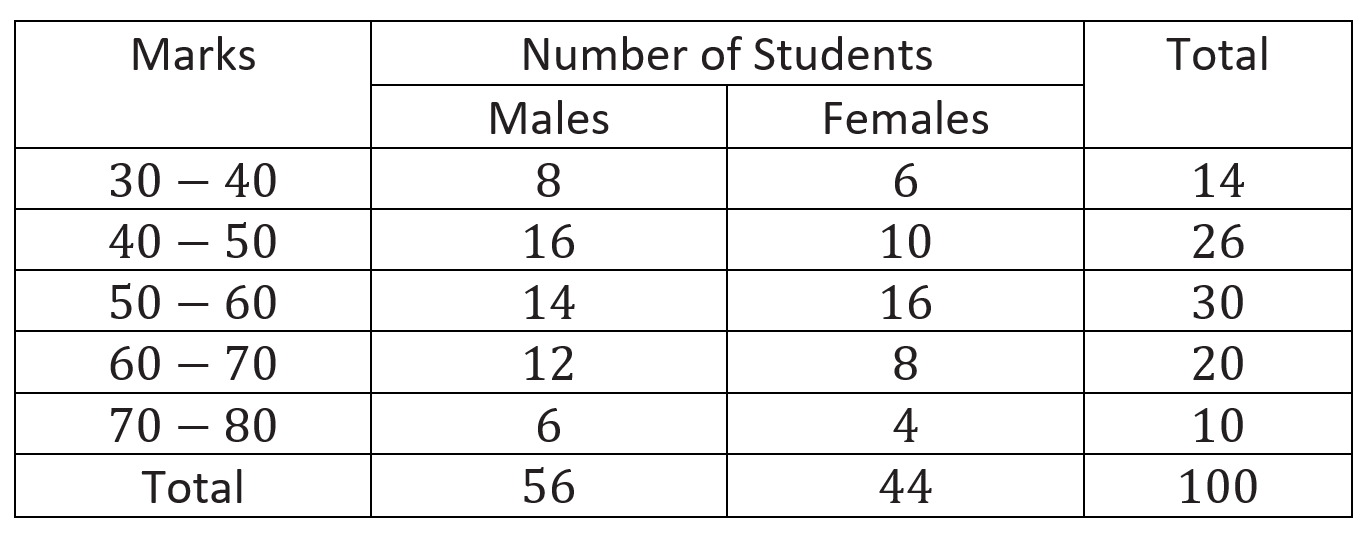
\includegraphics[width=10cm,height=4cm]{158.png}
 \vspace{2mm} 

 \end{questions}
\end{document}